\documentclass{ctexart}
\usepackage{graphicx}
\usepackage{tikz}
\usepackage{caption}
\usepackage{float}
\usepackage{amsmath}
\usepackage{fancyhdr}
\usepackage{xunicode-addon}
\usepackage{booktabs}
\usepackage{listings}
\usepackage{hyperref}
\usepackage{amssymb}
\usepackage[a4paper,hmargin=1.25in,vmargin=1in]{geometry}

% Add the TikZ library "bayesnet"
\usetikzlibrary{bayesnet}

% !TeX program = xelatex
\lstdefinestyle{mystyle}{
  basicstyle=\ttfamily\footnotesize,
  breakatwhitespace=false,         
  breaklines=true,                 
  captionpos=b,                    
  keepspaces=true,                 
  numbers=left,                    
  numbersep=5pt,                  
  showspaces=false,                
  showstringspaces=false,
  showtabs=false,                  
  tabsize=2
}

\lstset{style=mystyle}

\title{\begin{figure}[H]
	\centering 
	\includegraphics[height=7cm,width=14cm]{E:/Pictures/中科大.jpg}
	\end{figure}\Huge\textbf{Homework 3}\\\huge{Bayesian Network}}
\date{}
\punctstyle{banjiao} 
\pagestyle{fancy}
	\fancyhead[C]{\LARGE\textbf{Homework 3}}
	\fancyhead[L]{}
	\fancyhead[R]{}
	\fancyfoot[C]{\thepage}
\begin{document}
	\maketitle
	\thispagestyle{empty}
	
	\[\makebox{\Large{姓名:\underline{\makebox[5cm]{高茂航}}}}\]
	
    \[\makebox{\Large{学号:\underline{\makebox[5cm]{PB22061161}}}}\]
	
	$$\makebox{\Large{日期:\underline{\makebox[5cm]{2024.6.1}}}}$$
	
	\clearpage

	\pagenumbering{arabic}

	\section{概率推断[25\%]}
	\subsection{}
	\begin{figure}[h]
		\centering
		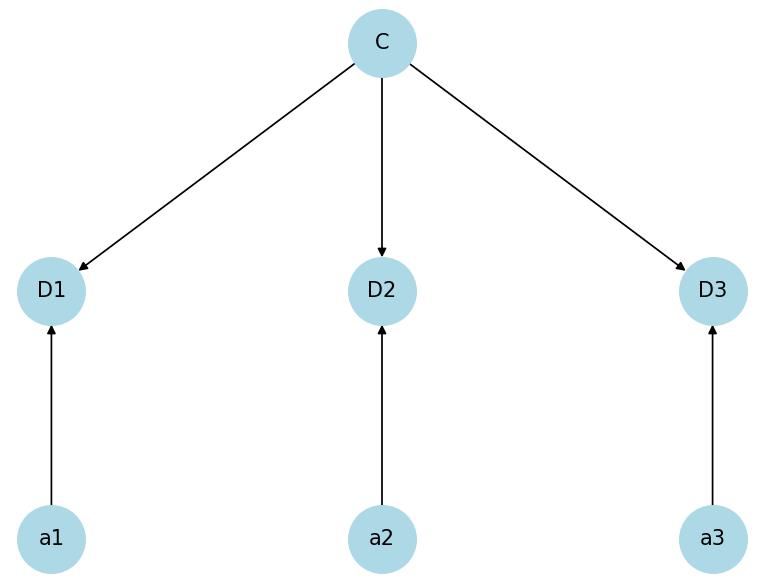
\includegraphics[height=6cm,width=10cm]{1.png}
		\end{figure}
		\subsection{}
		$\because D_t$ 只依赖于C和$a_t$,

		$\therefore P(C = c, D_1 = d_1, D_2 = d_2, D_3 = d_3) = P(C = c)P(D_1 = d_1 | C = c, a_1) P(D_2 = d_2 | C = c, a_2) P(D_3 = d_3 | C = c, a_3)$
		\subsection{}
		\begin{align*}
			P(C = c|D_1 = d_1, ..., D_t = d_t) &= \frac{P(C = c, D_1 = d_1, ..., D_{t-1}= d_{t-1}, D_t = d_t)}{P(D_1 = d_1, ..., D_{t-1} = d_{t-1}, D_t = d_t)}\\
			&= \frac{P(C = c)P(D_1 = d_1|C=c)P(D_2 = d_2|C=c) ...P(D_t = d_t|C=c)}{P(D_1 = d1, ..., D_{t-1} = d_{t-1}, D_t = d_t)}\\
			&= \frac{P(C = c,D_1 = d_1, . . . , D_{t-1} = d_{t-1})P(D=d_t|C = c)}{P(D_1 = d_1, ..., D_{t-1} = d_{t-1}, D_t = d_t)}\\
			&= \frac{P(C = c|D_1 = d_1, ..., D_{t-1} = d_{t-1})P(D=d_t|C = c)}{P(D_t=d_t|D_1 = d_1, . . . , D_{t-1} = d_{t-1})}\\
			& \propto P(C = c|D_1 = d_1, ..., D_{t-1} = d_{t-1})P(D=d_t|C = c)
		\end{align*}
		
		\subsection{}
		\begin{lstlisting}[language=Python]
			for i in range(self.belief.getNumRows()):
				for j in range(self.belief.getNumCols()):
					dist = math.sqrt((agentX - util.colToX(j))**2 + (agentY - util.rowToY(i))**2)
					prob = util.pdf(dist, Const.SONAR_STD, observedDist)
					self.belief.setProb(i, j, self.belief.getProb(i, j) * prob)
			self.belief.normalize()
			\end{lstlisting}

		\section{转移概率[25\%]}
		\subsection{}
		\begin{figure}[H]
			\centering
			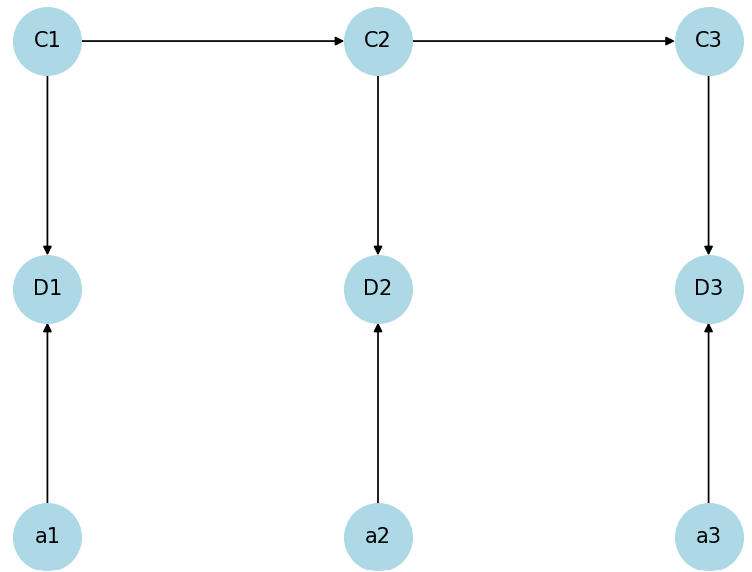
\includegraphics[height=6cm,width=10cm]{2.png}
			\end{figure}
			\subsection{}
			$\because D_t$ 依赖于$C_t$和$a_t$,且$C_t$依赖于$C_{t-1}$,
			
			$\therefore P(C_1 = c_1, C_2 = c_2, C_3 = c_3, D_1 = d_1, D_2 = d_2, D_3 = d_3) =P(C_1 = c_1) P(D_1 =d_1 | C_1 = c_1, a_1) P(C_2 = c_2 | C_1 = c_1) P(D_2 = d_2 | C_2 = c_2, a_2) P(C_3 = c_3| C_2 = c_2) P(D_3 =d_3| C_3 = c_3, a_3)$
			\subsection{}
			\begin{align*}
				P(C_{t+1} = c_{t+1}|D_1 = d_1, ..., D_t = d_t) 
				&= \frac{P(C_{t+1} = c_{t+1}, D_1 = d_1, ..., D_{t-1}= d_{t-1}, D_t = d_t)}{P(D_1 = d_1, ..., D_{t-1} = d_{t-1}, D_t = d_t)}\\
				&= \sum\limits_{c_t}\frac{P(C_{t+1} = c_{t+1}, C_t = c_t, D_1 = d_1, ..., D_{t-1}= d_{t-1}, D_t = d_t)}{P(D_1 = d_1, ..., D_{t-1} = d_{t-1}, D_t = d_t)}\\
				&= \sum\limits_{c_t}\frac{P(C_t = c_t,D_1 = d_1, . . . , D_t = d_t)P(C_{t+1}=c_{t+1}|C_t = c_t, ..., D_t = d_t)}{P(D_1 = d_1, ..., D_{t-1} = d_{t-1}, D_t = d_t)}\\
				&= \sum\limits_{c_t}\frac{P(C_t = c_t,D_1 = d_1, . . . , D_t = d_t)P(C_{t+1}=c_{t+1}|C_t = c_t)}{P(D_1 = d_1, ..., D_{t-1} = d_{t-1}, D_t = d_t)}\\
				& \propto\sum\limits_{c_t} P (C_t = c_t|D_1 = d_1, …, D_t = d_t)P(C_{t+1}=c_{t+1}|C_t=c_t)
			\end{align*}
			\subsection{}
			\begin{lstlisting}[language=Python]
				newBelief = util.Belief(self.belief.getNumRows(), self.belief.getNumCols(), 0)
        for oldRow in range(self.belief.getNumRows()):
            for oldCol in range(self.belief.getNumCols()):
                grid = self.belief.grid[oldRow][oldCol]
                for newRow in range(self.belief.getNumRows()):
                    for newCol in range(self.belief.getNumCols()):
                        transProb = self.transProb.get(((oldRow, oldCol), (newRow, newCol)), 0)
                        newBelief.addProb(newRow, newCol, grid * transProb)
        newBelief.normalize()
        self.belief = newBelief
				\end{lstlisting}
	
	\section{是哪辆车?[30\%]}
	\subsection{}
	\begin{align*}
		p(c_{11}, c_{12}|e_{1}) 
		&\propto p(C_{11} = c_{11}, C_{12} = c_{12},E_{1} = e_{1})\\
		&= p(c_{11}, c_{12})p(e_{1},e_{2}|c_{11}, c_{12})\\
		&= \frac{1}{2}p(c_{11})p(c_{12})[p(D_{11}=e_{11}|c_{11})p(D_{12}=e_{12}|c_{12})+p(D_{11}=e_{12}|c_{11})p(D_{12}=e_{11}|c_{12})]\\
		&= \frac{1}{2}p(c_{11})p(c_{12})[p_{N}(e_{11}; \lVert a_{1} - c_{11} \rVert^{2}, \sigma^{2})p_{N}(e_{12}; \lVert a_{1} - c_{12} \rVert^{2}, \sigma^{2})\\
		&\quad + p_{N}(e_{12}; \lVert a_{1} - c_{11} \rVert^{2}, \sigma^{2})p_{N}(e_{11}; \lVert a_{1} - c_{12} \rVert^{2}, \sigma^{2})]
		\end{align*}
	\subsection{}
	设循环群$$g=\binom{1,2,\dots ,K}{2,3,\dots ,1}$$
	则$z_t\in \{g^n|n=0, 1, ..., K-1\}$,用于表示在每个时间步 t,传感器返回的车辆位置列表相对于真实位置列表的偏移量,即
	$e_t=z_t(c_t)$。
	\begin{align*}
	p(c_{t} | c_{t-1}) 
	&=\frac{p(c_{t} ,c_{t-1})}{p(c_{t-1})} \\
	&= \sum\limits_{z_t}\frac{p(c_{t} ,c_{t-1}, z_{t})}{p(c_{t-1})} \\
	&= \sum\limits_{z_t}\frac{p(c_{t} ,c_{t-1}, z_{t})p(c_{t-1}, z_{t})}{p(c_{t-1}, z_{t})p(c_{t-1})}\\
	&= \sum\limits_{z_t} p(c_{t} |c_{t-1}, z_{t})p(z_{t}|c_{t-1})\\
	& =\frac{1}{K}\sum\limits_{z_t} p(c_{t} |c_{t-1}, z_{t})\\
	& =\frac{1}{K}\sum\limits_{z_t} p(z_{t}^{-1}(e_t) |z_{t-1}^{-1}(e_{t-1}), z_{t})
\end{align*}
	\subsection{}
	\begin{figure}[H]
		\centering
		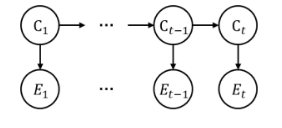
\includegraphics[height=3cm,width=6cm]{3.png}
		\caption{贝叶斯网络}
		\end{figure}
因为$E_t$由$C_t$和$Z_t$确定,且$Z_t$全为均匀分布(概率密度为1/K),因此上图没有画$Z_t$。

算法描述如下:

	1. 前向

	$$F_{1}(c_{1})=P(C_{1}=c_{1})P(E_{1}=e_{1}|C_{1}=c_{1})
	=\frac{1}{4}P(C_{1}=c_{1})$$
	\begin{align*}
	F_{i}(c_{i})&=\sum_{C_{i-i}}F_{i-1}(C_{i-1})P(C_{i}=c_{i}|C_{i-1})P(E_{i}=e_{i}|C_{i}=c_{i})\\
	&=\frac{1}{4}\sum_{C_{i-i}}F_{i-1}(C_{i-1})P(C_{i}=c_{i}|C_{i-1})
	\end{align*}

	2. 后向
	
	$$B_{T}(c_{T})=1$$
	$$B_{i}(c_{i})
	=\frac{1}{4}\sum_{B_{i+i}}F_{i+1}(C_{i+1})P(C_{i}
	=c_{i}|C_{i+1})$$

	3. 计算概率
	$$P(c_{t}|e_{1},...,e_{T})
	=\frac{F_{i}(c_{i}) B_{i}(c_{i})}{\sum\limits_{C_{t}}F_{i}(C_{i})B_{i}(C_{i})}$$
	\subsection{}
	
精确推理试图直接计算出概率分布的完整表达式,因而耗时较久;
相比之下粒子滤波方法更加高效,且在多车辆时error值更低、胜率更高。
因为粒子滤波方法只关注了概率较大的区域,且由于采样时会减少对小概率区域的权重,
因此小概率区域对大概率区域的影响不断减小,进而提高了准确度。

	\section{模型学习[10\%]}
	\subsection{}
	\begin{table}[H]
		\centering
		\caption{E step}
		\begin{tabular}{|c|c|c|c|c|c|}
		\hline
		$\mathrm{X_1}$ & $\mathrm{X_2}$ & $\mathrm{Z_1}$ & $\mathrm{Z_2}$ & $\mathrm{P}(\mathrm{X_1},X_2,Z_1,Z_2)$ & $\mathrm{q}((\mathrm{Z_1},Z_2))$ \\
		\hline
		true & false & true & true & $0.2646$ & $0.628$ \\
		\hline
		true & false & true & false & $0.0648$ & $0.154$ \\
		\hline
		true & false & false & true & $0.028$ &$0.066$ \\
		\hline
		true & false & false & false & $0.064$ &$0.152$ \\
		\hline
		true & true & true & true & $0.1134$ & $0.356$ \\
		\hline
		true & true & true & false & $0.0972$ & $0.305$ \\
		\hline
		true & true & false & true & $0.012$ & $0.038$ \\
		\hline
		true & true & false & false & $0.096$ & $0.301$ \\
		\hline
		\end{tabular}
	\end{table}
	\begin{table}[H]
		\centering
		\caption{M step}
		
		\begin{tabular}{|c|c|c|}
		\hline
		$\text{Z}_1$ & $\text{count}$ & $p_{Z_1}(Z_1)$ \\
		\hline
		true & $1.443$ & $0.72$ \\
		\hline
		false & $0.557$ & $0.28$ \\
		\hline
		\end{tabular}
	\end{table}	
	\begin{table}[H]
		\centering
		\begin{tabular}{|c|c|c|c|}
		\hline
		$\text{Z}_1$ & $\text{Z}_2$ & $\text{count}$ & $p_{Z_2}(Z_2|Z_1)$ \\
		\hline
		true & true & $0.984$ & $0.68$ \\
		\hline
		true & false & $0.459$ & $0.32$ \\
		\hline
		false & true & $0.104$ & $0.19$ \\
		\hline
		false & false & $0.453$ & $0.81$ \\
		\hline
		\end{tabular}
	\end{table}	
	\section{反馈[10\%]}
	本次实验花了近一周的空闲时间,主要是在第三部分卡了很久,经过讨论,得知应该是题目本身就有问题。
	
	



	

\end{document}